%!TEX root = skripsi.tex
%-----------------------------------------------------------------------------%
\chapter{\babDua}
This chapter focuses on literature study on three aspects including language models, deep learning, and semantic role labeling. In language model section, Part-of-Speech tag (POS tag) and word embedding are described. Deep learning section focuses on the architecture widely used for sequence labeling problem. Finally, we explain semantic role labeling in the last section, including the semantic roles definition, annotation corpus, problem definitions, common features, and the historical perspectives.
%-----------------------------------------------------------------------------%
%-----------------------------------------------------------------------------%
\section{Language Models}
This section explains the language models usually used in Natural Language Processing (NLP) applications. We first describe the traditional yet important language model, Part-of-Speech tag (POS tag), followed by the so-called word embedding that is often used in recent NLP systems.

\subsection{Part-of-Speech Tag (POS Tag)}
Part-of-Speech (POS) tag defines the class of a word. Some examples of POS tag are noun, verb, adverb, and adjective. POS tags are useful because of the large amount of information they give about a word and
its neighbors. Knowing whether a word is a noun or a verb tells us a lot about likely neighboring words (nouns are preceded by determiners and adjectives, verbs by nouns) and about the syntactic structure around the word (nouns are generally part of noun phrases).

\subsection{Word Embedding}
Word representation is an important feature when one wants to build deep learning model for NLP tasks. The idea is to convert words into vectors. There are two approaches for this vector representation, which are traditional and word embedding approach. Traditional approach uses one-hot vectors for the representation, meanwhile word embedding approach uses real values vectors that contain information about the words.

In the traditional approach, the vectors are retrieved based on the index of the word found in the dictionary. The dictionary consists of the word and its index. Suppose that we have four words: \textit{I, eat, chicken, you}. Each of these words has their own index, with \textit{I}:0, \textit{eat}:1, \textit{chicken}:2, \textit{you}:3. These indices will represent the one-hot vectors for the words. For instance, word with index 0 has a one-hot vector [1, 0, 0, 0], word with index 1 has a one-hot vector [0, 1, 0, 0], and so on. The length of the vector is determined by the size of our dictionary. In this case, the size of our dictionary is 4, hence the length of the vector is also 4. 

This approach, however, has a drawback since the vector representation is sparse. As we just give the index to the all the words based on the dictionary, it does not really represent an important information from the words. For instance, the word \textit{chicken} and \textit{beef}, though have similarity as they are eatable, can be represented by two far indices, say 1 and 100. This representation therefore does not capture the similarity between those words. 

To address this issue, there is another better word representation approach: the so-called word embedding. Word embedding is designed to represent word with a dense, low dimension, real-values vector. For example, the word \textit{chicken} is mapped into a vector [0.28, 0.31, -0.17, ..., 0.89]. With this representation, word embedding transforms similar words to similar vectors. From the previous example, the word \textit{chicken} and \textit{beef} will most likely have vectors that are close to each other.

There has been a lot of research on word embedding, such as Word2Vec~\citep{mikolov2014word2vec} and Glove~\citep{pennington2014glove}. In this section, we only explain Word2Vec since we will use this later in our research. Word2Vec uses unsupervised approach so that we only need a lot of unlabeled data for building word embedding model. Basically, Word2Vec uses neural networks architecture to train the unsupervised data. Word2Vec is able to learn and classify words based on their similarity and represent it in the vector space.

\begin{figure}
	\centering
	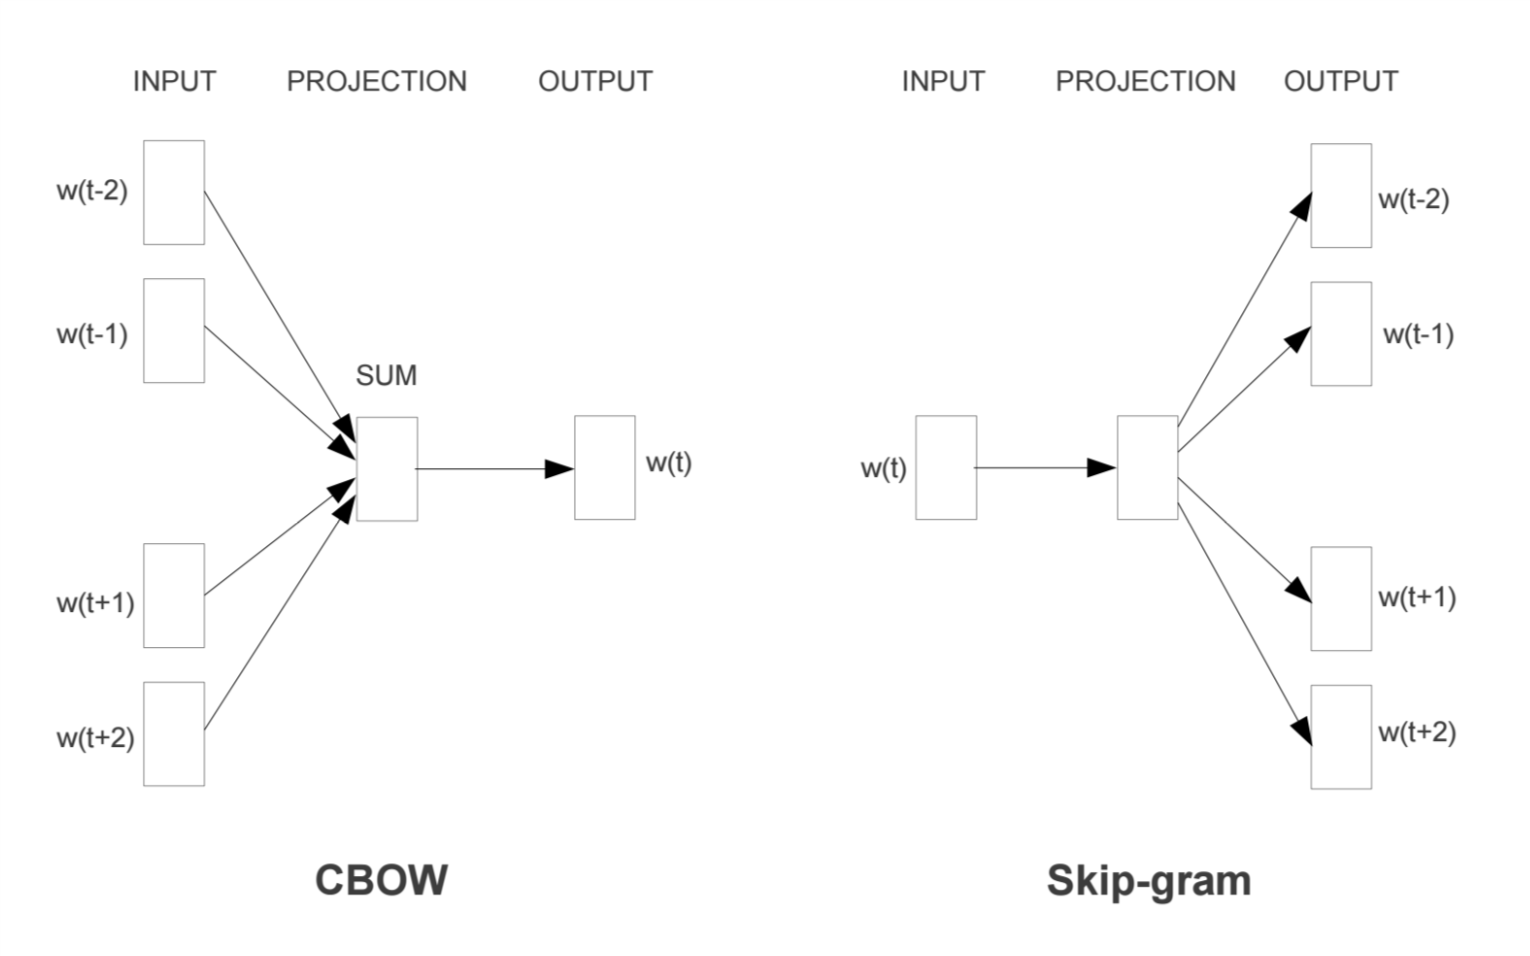
\includegraphics[width=0.85\linewidth]{images/word2vec}
	\caption{Arsitektur Word2Vec}
	\label{fig:word2vec}
\end{figure}

Word2Vec has two architectures, namely Context Bags of Words (CBOW) and Skipgram, as illustrated in Figure~\ref{fig:word2vec}. In CBOW, the model learns to predict a word based on its neighboring words. Therefore, the input layer is represented with the bag-of-words. In contrast, Skipgram architecture aims to predict the neighbouring words based on a given word. The advantage of CBOW is that it can be used for training a huge amount of data, while Skipgram is best for capturing the average co-occurance from two words from the data.

Both architectures mainly aims to build language model, however, one does not need the whole trained model for having the word embedding representation. Instead, we only need to extract the weight matrix used for converting words into vectors from the model. This weight matrix is the word embedding model that we use for transforming the words into the dense vectors.

\section{Deep Learning}
Deep learning is a branch of machine learning that has multiple layers inside the model. Deep learning is able to extract implicit features in a high, abstract level~\citep{lecun2015deep}. Deep learning model has proved to produce robust performance in a variety of reserach, including computer vision and natural language processing.

Deep learning is basically a neural networks model with deeper hidden units. Neural networks model is based on how the neuron works inside human brain. Neurons with deep hidden units are then able to extract features in a abstract level~\citep{bengio2007scaling}. The deep learning structure consists of input layer, hidden layer, and output layer. The input layer is where the data being fed into the model, while output layer is the result of the model. The important layer here is the hidden layer in which a linear and/or non-linear functions are approximated in order to get the best predicted outputs.

Deep learning model has proved to give outstanding performances in supervised learning~\citep{Goodfellow-et-al-2016-Book}. A model with deeper layer will learn more implicit features out of the training data. There are a lot of deep learning models that have been proposed, some of which are Recurrent Neural Networks~\citep{elman1990finding} and Convolutional Neural Networks. Each of the deep learning models is designed to fulfill specific computation needs.

\subsection{Recurrent Neural Networks}
Recurrent Neural Networks, shortened as RNN, is one of deep learning models designed for processing sequential data. There are some varieties of RNN, including the one proposed by~\cite{elman1990finding} and~\cite{jordan1986attractor}. Since it is designed for processing sequential data, it has a nature advantage for modeling the sequence labeling problem. Suppose that we have sequence of inputs, RNN will take each input in a time step $t$ to process it in a function. Figure~\ref{fig:simplernn} shows a general RNN.

\begin{figure}
	\centering
	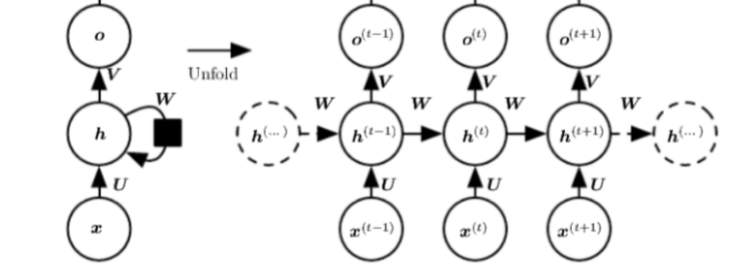
\includegraphics[width=0.80\linewidth]{images/simplernn}
	\caption{A simple Recurrent Neural Networks (RNN). (left) folded RNN. (right) unfolded RNN}
	\label{fig:simplernn}
\end{figure}

The left picture illustrates the folded RNN model applied to all time steps. Note that the black rectangle represents one time step delay, meaning that that input is coming from the output of the previous time step. 

The right picture shows the unfolded RNN that is more intuitive since it visualizes the time steps. There are three layers in every time step t, which are input, hidden, and output layers. The input layer is for the input representations. In the hidden layer, it contains information from the input layer as well as those coming from hidden layers in the previous time steps. The output layer consists of the output of the model. These three layers are in a form of vectors. In every time step $t$, RNN has an input layer $ \vec{x(t)} \in {\rm I\!R^{A}} $, hidden layer $ \vec{h(t)} \in {\rm I\!R^{H}} $, and output layer $ \vec{o(t)} \in {\rm I\!R^{B}} $. The values of $A$, $H$, and $B$ represent the length of the input vector, the number of unit in a hidden layer, and the length of the output vector, respectively. There are three parameters that will be trained, which are $U$, $V$, and $W.$ These parameters are the weight matrices for connecting two layers. $ U \in {\rm I\!R^{H \times A }}$ connects input layer with hidden layer (input-hidden), $ W \in {\rm I\!R^{H \times H}}$ connects hidden layer with the previous hidden layer (hidden-hidden), and $ V \in {\rm I\!R^{B \times H}}$ connects hidden layer with output layer (hidden-ouput). These parameters are time-distributed, meaning that they are shared across time steps. 

Every input layer $ \vec{x(t)} $ is mapped into output layer $ \vec{o(t)} $ in every time step $t$. In the middle of the process, the model calculates the hidden layer $ \vec{h(t)} $ from two layers, $ \vec{x(t)} $ and $ \vec{h(t-1)} $. The output layer $ \vec{o(t)} $ then is retrieved by performing a function to the hidden layer h(t). The general equations for RNN are presented as follows:
\begin{equation}
\label{eq:rnnot}
\vec{o(t)} = f2(V \cdot \vec{h(t)} + \vec{c})
\end{equation}

\begin{equation}
\label{eq:rnnht}
\vec{h(t)} = f1(U \cdot \vec{x(t)} + W \cdot \vec{h(t-1)} + \vec{b})
\end{equation}

Where $ \vec{h(0)} = f1(U \cdot \vec{x(0)}) $.

Note that there are two additional parameters to train, which are the bias vectors $\vec{b}$ and $\vec{c}$. In Equation~\ref{eq:rnnht}, the input $\vec{x(t)}$ and $\vec{h(t-1)}$ are weighted by matrices $U$ and $W$ respectively, added by a bias vector $\vec{b}$. The result is then inserted to an activation function $f1$ in order to produce hidden layer $\vec{h(t)}$. In the Equation~\ref{eq:rnnot}, $\vec{h(t)}$ is multiplied by the weight matrix $V$ and added by a bias vector $\vec{c}$ before being processed by the activation function $f2$ to produce $\vec{o(t)}$. The examples of activation function $f1$ and $f2$ are tanh and softmax.

Based on this illustration, there are two main characteristics of RNN:
\begin{enumerate}
	\item It has a cycle in the graph for every time step. Hidden layer $\vec{h(t-1)}$  will be one of the inputs for forming $\vec{h(t)}$ .
	\item It has shared parameters across time steps.
\end{enumerate}

Figure~\ref{fig:fulrnn} illustrates a more complete RNN model on how it is being trained.

\begin{figure}
	\centering
	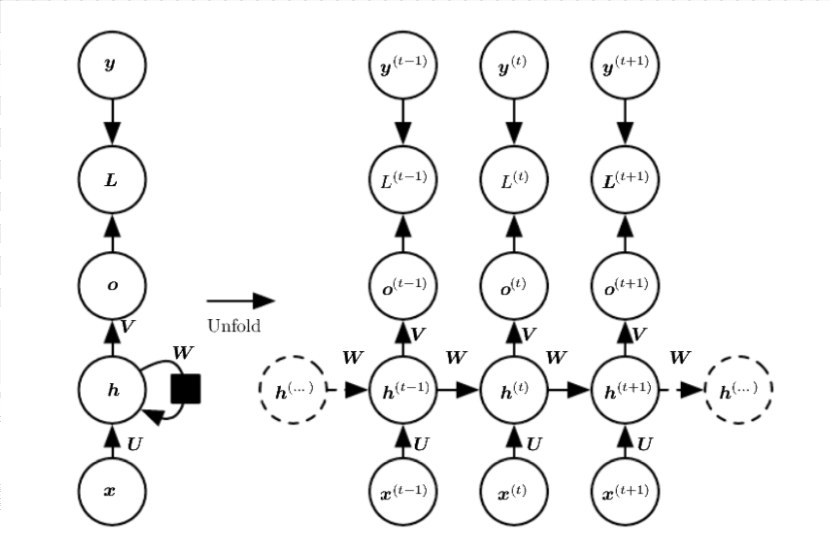
\includegraphics[width=0.80\linewidth]{images/fullrnn}
	\caption{A Recurrent Neural Networks (RNN). (left) folded RNN. (right) unfolded RNN}
	\label{fig:fulrnn}
\end{figure}

The goal of training the model is to find the estimated values of parameters $W$, $U$, $V$, $\vec{b}$, and $\vec{c}$ which produce output $\vec{o(t)}$ as close as the expected output $\vec{y(t)}$ in the training data. 

The loss function $L$ measures the difference between the predicted output $\vec{o(t)}$ and the expected output $\vec{y(t)}$ in every time step t. The smaller the difference, the better the model. The machine thus has to minimize the result of loss function as small as possible. The parameters $W$, $U$, $V$, $\vec{b}$, and $\vec{c}$ are unknown in the beginning. At first, these parameters are initiated randomly. For every iteration, called epoch, the machine aims to learn the best values for each parameter.

The way to do so is by computing the gradient for each iteration. The idea behind computing the gradient values is to show us which parameter setting that brings us into smaller loss function result. By having this information, the machine then sets the better values for each parameter in the next iteration in order to reduce the loss function. From one iteration into another, the machine will find better parameter values to minimize the loss function. The learning method based on the gradient information is called optimization algorithm. Some optimization algorithms available are Stochastic Gradient Descent (), Adam (Kingma and Ba, 2014), and RMSProp (Hinton, 2012).

\subsection{Long Short-Term Memories}
Regular RNN has an issue called vanishing and exploding gradient problem. The RNN architecture repeatedly uses the same parameters for each time steps. Suppose that we use $W$ as the parameter for each time step between the hidden units. After $t$ time steps, the matrix would be multiplied $t$ times, hence it is the same as multiplying the hidden units with Wt. Assuming that $W$ has an eigen-decomposition $W = X \cdot diag(\lambda) \cdot X^{-1}$, $W^{t}$ is equal to:
\begin{equation}
W^{t} = (X \cdot diag(\lambda) \cdot X^{-1})^{t} = (X \cdot diag(\lambda)^{t} \cdot X^{t})
\end{equation}

The eigenvalues $\lambda$ in $diag(\lambda)$ will either vanish if they are less than 1 in magnitude or explode if they are greater than 1 in magnitude. The gradient counted in each time step is aligned with the eigenvalues. Hence, the gradient may also vanish or explode. This is what we called as vanishing and exploding gradient problem. When the gradient vanishes, it is hard for the machine to find the direction to reduce the cost function. In the case of exploding gradient, the learning algorithm will become unstable.

To address this issue, there are solutions proposed such as leaky units (Mozer, 1992), simulated annealing and discrete error propagation (Bengio et al., 1994), time delays (Lang et al., 1990), and hierarchical sequence compression (Schmidhuber et al., 2007). Among these approach, one of the most robust solutions is the Long Short Term Memories (LSTM) (Hochreiter et. al., 1997). 

The modification added in LSTM to address the issue is by using gates. It is basically RNN, but the nonlinear units in the hidden layer is replaced by the memory blocks. One nonlinear unit $tanh$ in RNN is replaced by more complex memory blocks in LSTM. Besides the hidden layer $\vec{h(t)}$, LSTM also has $\vec{m(t)}$ which is called memory cells.  The idea of LSTM is to learn when to forget or remember the memory from previous time steps through multiplicative gates. It thus prevents the vanishing and exploding gradient problem. For example, if the input gate is closed, then the memory will be unchanged.

\begin{figure}
	\centering
	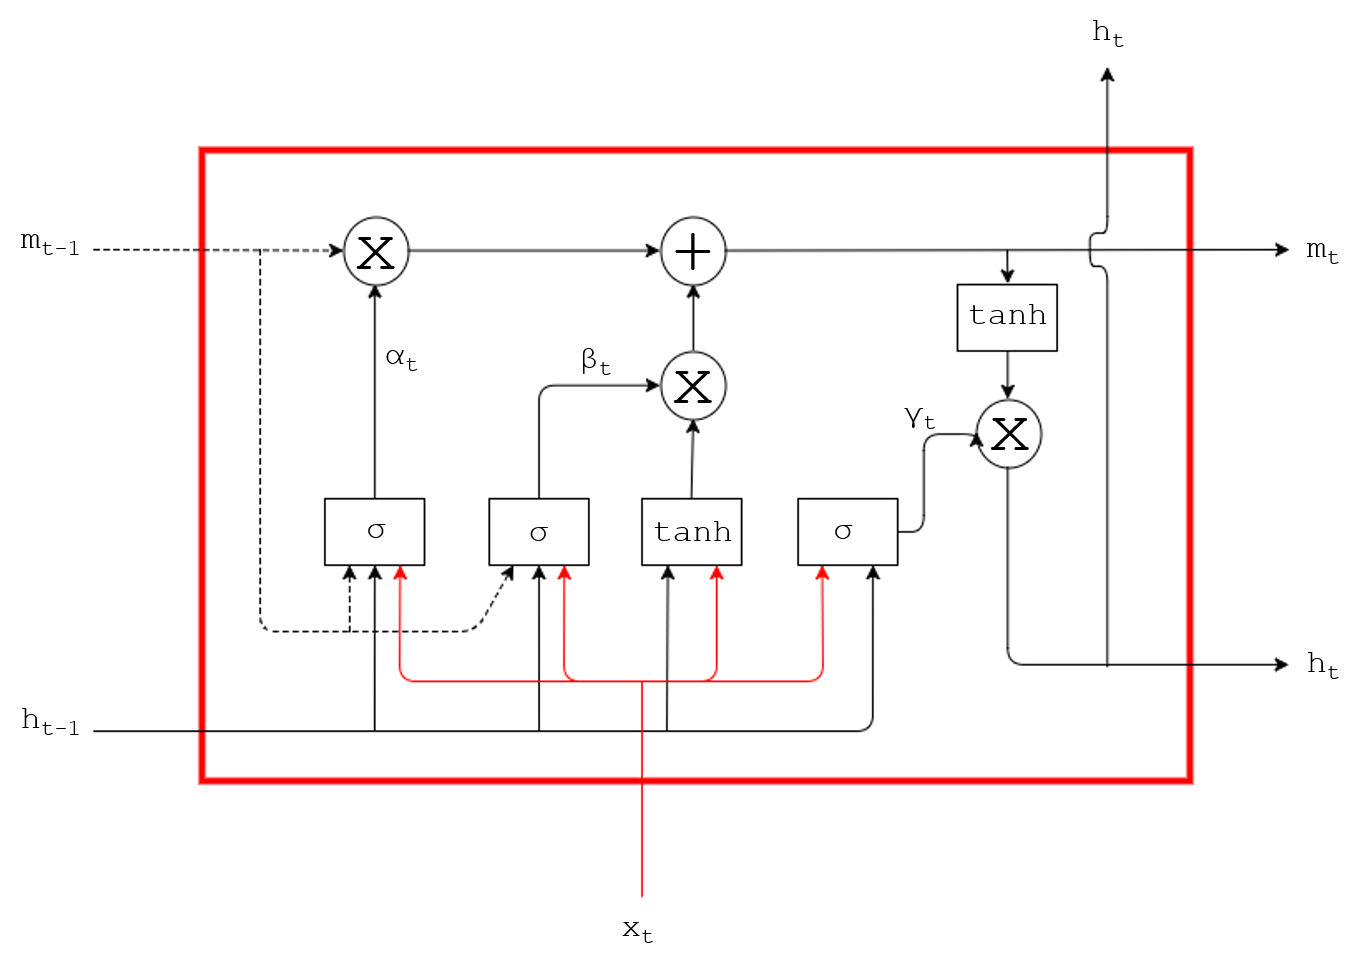
\includegraphics[width=1.0\linewidth]{images/lstm}
	\caption{One memory block in LSTM}
	\label{fig:lstm}
\end{figure}

Figure~\ref{fig:lstm} illustrates a one block memory in LSTM. There are three main gates, which are forget gate, input gate, and output gate. These gates are responsible to determine whether an information is added, kept, or deleted in a cell. Each gate has sigmoid layer and element-wise operations. The sigmoid layer converts the input into a probability between 0 and 1. This probability describes the gate behavior towards the input, whether to accept it (probability close to 1) or not (probability close to 0). 

The equations of the sigmoid layers for each of the gates are explained as follows:
\begin{enumerate}
	\item \textit{Forget Gate}\\
	This gate is responsible to determine how much the information from the past should be kept in the memory. The equation of the forget gate is given as follows:
	\begin{equation}\label{eq:forget_lstm}
	\alpha_{t}=\sigma(W_{x\alpha}\cdot x_{t}+W_{h\alpha}\cdot~h_{t-1}+W_{m\alpha}\cdot~m_{t-1})
	\end{equation}
	
	\item \textit{Input Gate}\\
	This gate is responsible to determine how much the current information x(t) should be kept in the memory. The equation of the input gate is given as follows:
	\begin{equation}\label{eq:input_lstm}
	\beta_{t}=\sigma(W_{x\beta}\cdot x_{t}+W_{h\beta}\cdot~h_{t-1}+W_{m\beta}\cdot~m_{t-1})
	\end{equation}
	
	\item \textit{Output Gate}\\
	This gate is responsible to determine the output of a time step based on current cell state. The equation of the output gate is given as follows:
	\begin{equation}\label{eq:output_lstm}
	\gamma_{t}=\sigma(W_{x\gamma}\cdot x_{t}+W_{h\gamma}\cdot~h_{t-1}+W_{m\gamma}\cdot~m_{t-1})
	\end{equation}
	
\end{enumerate}

In every time step $t$, the equations for computing cell state $m(t)$ and hidden layer $h(t)$ are presented as follows:
\begin{equation}\label{eq:mt}
m_{t}=\alpha_{t} (\times) m_{t-1} + \beta_{t} (\times) tanh(W_{xm} \cdot x_{t} + W_{hm} \cdot h_{t-1}))
\end{equation}
\begin{equation}\label{eq:ht}
h_{t}=\gamma_{t} (\times) tanh(m_{t})
\end{equation}

\section{Semantic Role Labeling}
Semantic role labeling (SRL) is a task in Natural Language Processing to assign semantic roles for each argument for each predicate in given input sentence. In this section, the definition of semantic roles and the most commonly used annotation corpus for SRL are explained. In the end, the details on the semantic role labeling task are described.

\subsection{Semantic Roles}
Semantic roles are the representations that express the abstract role of the arguments of a predicate can take in the event~\citep{jurafsky2000speech}. When it comes to understanding natural language, one would want to understand the events and their participants of a given input sentence. In this case, the events refer to the predicate and the participants refer to the argument. Table~\ref{tab:examplesrl1} illustrates the connection between a predicate and its arguments.

\begin{table}
	\centering
	\caption{An example predicate and its arguments}
	\label{tab:examplesrl1}
	\begin{tabular}{|ccc|}
		\hline
		\underline{Andy} & \underline{eats} & \underline{fried chicken} \\
		Argument & Predicate & Argument \\
		\hline
	\end{tabular}
\end{table}

In this example, eat is the predicate with Andy and fried chicken as its argument. With this point of view, the predicate can be seen as the center of the sentence, followed by the arguments that depend on it.

Knowing the predicate and its arguments is not enough to understand the sentence since the roles of the arguments towards the predicate are unknown. In the previous example, it will be more meaningful to differentiate that Andy is the Eater and fried chicken is the EatenThing. Eater and thing eaten are the examples of semantic roles for the predicate eat. These semantic roles could be used to identify the roles of the arguments regardless its position in the sentence. The previous example could be represented in two ways, as presented in Table~\ref{tab:examplesrl2}

\begin{table}
	\centering
	\caption{An example predicate and its deep roles}
	\label{tab:examplesrl2}
	\begin{tabular}{|ccc|}
		\hline
		\underline{Andy} & \underline{eats} & \underline{fried chicken} \\
		Eater & Predicate & EatenThing \\
		\hline
		\underline{The fried chicken} & is \underline{eaten} & by \underline{Andy} \\
		EatenThing & Predicate &  Eater \\
		\hline
	\end{tabular}
\end{table}

Both sentences represent the role of Andy and fried chicken as eater and thing eaten respectively, regardless of their position in the sentence as a subject or object.

There are many ways to define such semantic roles. From the examples above, the semantic roles are very specific for its predicate, known as deep roles~\citep{jurafsky2000speech}. Eater and ThingEaten are semantic roles for the predicate eat, Kicker and KickedThing are semantic roles for the predicate kick, and so on. In order to further knowing more about the semantics of these arguments, these semantic roles could be generalized into more abstract roles. Eater and Kicker have something in common: they are volitional actors having direct causal responsibility for the predicate. For this reason, thematic roles are introduced as a set of semantic roles designed to capture semantic commonality between Eater and Kicker~\citep{jurafsky2000speech}. With this in mind, Kicker and Eater can be represented as AGENT, which represents the abstract concept that is a volitional causer of an event (or predicate). On the other hand, EatenThing and KickedThing both represent the direct objects that are affected by the event. The semantic role for EatenThing and KickedThing is THEME.

Table~\ref{tab:examplesrl3} shows the thematic roles often used across computational papers~\citep{jurafsky2000speech}
\begin{table}
	\scriptsize
	\centering
	\caption{Examples of thematic roles}
	\label{tab:examplesrl3}
	\begin{tabular}{lll}
		\hline
		\textbf{Thematic Role} & \textbf{Definition} & \textbf{Example} \\
		\hline
		AGENT & The volitional causer of an event & \underline{The waiter} spilled the soup \\
		EXPERIENCER & The experiencer of an event & \underline{John} has a headache \\
		FORCE & The non-volitional causer of the event & \underline{The wind} blows debris \\
		THEME & The participant directly affected by an event & Benjamin Franklin broke \underline{the ice} \\
		RESULT & The end product of an event & The city built \underline{a requlation-size baseball diamond} \\
		CONTENT & The content of a propositional event & Mona asked \underline{"Did you met Mary Ann?"} \\
		INSTRUMENT & An instrument used in an event & He stunned catfish with \underline{a shocking device} \\
		BENEFICIARY & The beneficiary of an event & Ann Callahan makes hotel reservations for \underline{her boss} \\
		SOURCE & The origin of the object of a transfer event & I flew in \underline{from Boston} \\
		GOAL & The destination of an object of a transfer event & I drove \underline{to Portland} \\
		\hline
	\end{tabular}

\end{table}


\subsection{Annotation Corpus}
There are available annotated corpus for SRL consists of sentences labeled with semantic roles. Researchers are using these annotated corpus for building supervised machine learning model for SRL. The two most commonly used annotation corpus for SRL are Proposition Bank and FrameNet.

\subsubsection{Proposition Bank}
Proposition Bank~\citep{kingsbury2002treebank}, shortened as PropBank, is a corpus in which sentences are annotated with semantic roles. PropBank corpus is available for many languages, such as English, Chinese, Hindi, Arabic, Finnish, and Portuguese. The main approach used for its semantic roles grouping is based on proto-roles and verb-specific semantic roles. Every verb sense has its set of semantic roles with argument numbers rather than names, for example: Arg0, Arg1. Arg2, etc. Generally, Arg0 represents PROTO-AGENT while Arg1 represents PROTO-PATIENT. Other argument number representations may vary based on each verb sense.

The PropBank entries are called frame files. One example of the frame files for one sense of verb eat is presented as follows.
\\
\fbox{%
	\parbox{1.0\linewidth}{%
		\textbf{Frame File:}\\
		\textit{Eat.01}\\
		Arg0: Eater\\
		Arg1: Things Eaten\\
		Arg2: Instrument used\\
		\\
		\textit{Example:}\\
		Ex1: [Arg0 Andy] eats [Arg1 fried chicken] [Arg2 with spoon]\\
		Ex2: [Arg1 That fried chicken] is eaten by [Arg0 Andy] [Arg2 with spoon]
	}%
}
\\

For verb sense Eat.01, Arg0 acts as the Eater (PROTO-AGENT), and Arg1 represents the Things Eaten (PROTO-PATIENT). As we can see from the example above, we can infer the commonality between examples Ex1 and Ex2 regardless its structure, be it in a passive or active voice. In both examples, Andy is the Eater and fried chicken is the Things Eaten. In this frame file, there is also another argument, Arg2, that represents the instrument used by the Eater. In example Ex1 and Ex2, the instrument is spoon.

Other non-numbered arguments are available in PropBank, the so-called ArgMs, representing modifiers that could be used across frame files. Some examples of ArgMS include:
\\
\fbox{%
	\parbox{1.0\linewidth}{%
		TMP: When?\\
		LOC: Where?\\
		DIR: Where to/from?\\
	}%
}
\\

The next annotation corpus is called FrameNet which has different approach on how to group the set of semantic roles. Instead of using verb-specific, it uses frame-specific grouping.

\subsubsection{FrameNet}
FrameNet~\citep{baker1998berkeley} is an annotation corpus for semantic roles that are specific to a frame. In PropBank, the semantic roles are defined based on each sense of a verb. In contrast, a frame in FrameNet could include more than one predicate (verbs or nouns) that have the same background context. Each frame consists of two elements: 1.) A set of semantic roles related to this frame, and 2.) A set of predicates using the respective semantic roles.

One example is a frame called $\mathbf{change\_position\_on\_a\_scale}$ defined as:
\\
\fbox{%
	\parbox{1.0\linewidth}{%
		\texttt{This frame consists of words that indicate the change of an Item's position on a scale (the Attribute) from a starting point (Initial value) to an end point (Final value).} \\
	}%
}
\\

The set of semantic roles for a frame is divided into two roles: Core roles and Non-Core Roles. Core Roles are specific to a frame while Non-Core Roles are more general across frames (like ArgMs in PropBank). The set of semantic roles of the frame $\mathbf{change\_position\_on\_a\_scale}$ is explained as bellow:
\\
\fbox{%
	\parbox{1.0\linewidth}{%
		\textbf{Core Roles}\\
		ITEM: The entity that has a position on the scale.\\
		ATTRIBUTE: The ATTRIBUTE is a scalar property that the ITEM possesses\\
		DIFFERENCE: The distance by which an ITEM changes its position on the scale. FINAL STATE: A description that presents the ITEM's state after the change in the ATTRIBUTE's value as an independent predication.\\
		FINAL VALUE: The position on the scale where the ITEM ends up. \\
		INITIAL STATE: A description that presents the ITEM's state before the change in the ATTRIBUTE's value as an independent predication.\\
		INITIAL VALUE:The initial position on the scale from which the ITEM moves away. \\
		VALUE RANGE: A portion of the scale, typically identified by its end points, along which the values of the ATTRIBUTE fluctuate. \\
		\\
		\textbf{Non-Core Roles}\\
		DURATION SPEED GROUP\\
		The length of time over which the change takes place.\\
		The rate of change of the VALUE.\\
	}%
}
\\

For instance, the possible predicates of the frame change position on a scale are: \textit{rose, increase, fell}.

The example of semantic roles of the frame change position on a scale can be seen as follows:

[ITEM Oil] rose [ATTRIBUTE in price] [DIFFERENCE by 2\%]. 

[ITEM It] has increased [FINAL STATE to having them 1 day a month]. 

[ITEM Microsoft shares] fell [FINAL VALUE to 7 5/8]. 

[ITEM Colon cancer incidence] fell [DIFFERENCE by 50\%] [GROUP among men]

a steady increase [INITIAL VALUE from 9.5] [FINAL VALUE to 14.3] [ITEM in dividends]

a [DIFFERENCE 5\%] [ITEM dividend] increase... 

As we can see from the examples above, \textit{rose}, \textit{fell}, and \textit{increase} have the same set of semantic roles under the frame change position on a scale. Instead of defining the semantic roles for each verb sense one by one, FrameNet groups predicates (not limited to verbs) that have same semantic roles as one frame.

\subsection{Problem Definitions}
Semantic Role Labeling (SRL) is one of Natural Language Processing task which aims to automatically assign semantic roles for each constituent (argument) for each predicate in a sentence~\citep{jurafsky2000speech}. Current approach to solve this task is by using supervised machine learning. Given a labeled data, the machine learns from it and builds a generalization model. Researches often used PropBank or FrameNet corpus as the sources of annotated data. In this section, we describe the approaches to define the problem of SRL task, followed by the common features used for building supervised model for SRL.

There are two ways to see SRL problem, either as Classification or Sequence Labeling problem. Classification approach assigns semantic roles for each word independently. Meanwhile, Sequence Labeling approach traverses from assigning semantic role for the first word until the last one in a sentence sequentially. In Sequence Labeing, the next label (semantic role) prediction of time step t is dependent to labels predicted on previous time steps (1..t-1).

In classification approach approach, suppose that we have an input of \textit{n} words $w = (w_{1}, w_{2}, ..., w_{n})$. Each vector $w_{i}$ is classified into a label $y_{i}$ that represents the semantic role. The probabilities of the label in each time step $i$ is described as follows.
\begin{equation}
P(y_{i}|w_{i})
\end{equation}

In sequence labeling approach, suppose that we have an input of \textit{n} words $w = (w_{1}, w_{2}, ..., w_{n})$, the goal is to find the best label sequence $y = (y_{1}, y_{2}, ..., y_{n})$, with $y_{i}$ representing the semantic roles. The probabilities of the label in each time step $i$ is described as follows.
\begin{equation}
P(y_{i}|w_{i-l}, ..., w_{i+l},y_{i-l}, ..., y_{i+l})
\end{equation}

whereby \textit{l} is a small number. 

\subsection{Common Features for SRL}
The first set of features for SRL is proposed by Gildea and Jurafsky (2000). They are the first ones who used supervised machine learning approach to solve SRL. Over the years, many research proposed new set of features to improve the result, but they still used the basic features proposed by Gildea and Jurafsky (2000). The common features used for solving SRL task are:
\begin{enumerate}
	\item The predicate.\\
	Usually in a form of verb.
	\item The phrase type of the constituent.\\
	NP, PP, etc
	\item The headword of the constituent.\\
	The black bird. Headword: bird.
	\item The headword part of speech of the constituent. \\
	Example: NNP.
	\item The path of the parse tree from constituent to predicate. \\
	This is to represent the grammatical relationships between the constituent and the predicate.
	Example: NP S VP VBD
	\item The voice of the clause, active or passive.\\
	Example: I eat chicken rice (active), Chicken rice is eaten by me (passive).
	\item The binary linear position of the constituent from the predicate.\\
	Could be before or after the predicate.
	\item The subcategorization of the predicate\\
	Set of arguments that appear in the verb phrase VP.
	Example: NP and PP in 'VP -> VBD NP PP'
	\item The named entity type of the constituent\\
	Example: Organization, Person, Location
	\item The first and last words of the constituent.
\end{enumerate}

There are also other additional features that could be used for SRL, such as sets of n-grams inside the constituent. Another variation is to use dependency parser instead of syntactic parser for extracting features.

\subsection{Historical Perspectives}
SRL can be seen as either a classification or sequence labeling problem. The earlier research on SRL was conducted with the classification approach, meaning that each argument is being predicted independently from the others. Those research focused on how to extract meaningful features out of syntactic parsers~\citep{gildea2002automatic, gildea2002necessity, pradhan2005semantic}, such as the path to predicate and constituent type. This syntactic information plays a pivotal role in solving SRL problem~\citep{punyakanok2008importance} as it addresses SLR's long distance dependency~\citep{zhou2015end}. Thus, traditional SRL system heavily depends on the quality of the parsers. The analysis done by Pradhan et al. shows that most errors of the SRL system were caused by the parser's error~\citep{pradhan2005semantic}. In addition, those parsers are costly to build, since it needs linguistic experts to annotate the data. If we want to create an SRL system on another language, one should build a new parser all over again for it~\citep{zhou2015end}.

In order to minimize the number of hand-crafted features, Collobert et al. utilized deep learning for solving NLP tasks including Part-of-Speech Tagging (POS), Chunking (CHUNK), Named Entity Recognition (NER), and Semantic Role Labeling (SRL) with classification approach~\citep{collobert2011natural}. The research aims to prevent using any task-specific feature in order to achieve state-of-the-art performance. The word embedding is used as the main feature across tasks, combined with Convolutional Neural Networks (CNN) architecture to train the model. They achieve promising results for the POS Tagging and Chunking, while for SRL features from the parsers are still needed to achieve competitive results.

Different from the previous works, Zhou et al. view SRL as a sequence labeling problem in which the arguments are labeled sequentially instead of independently~\citep{zhou2015end}. They proposed an end-to-end learning of SRL using Deep Bi-Directional Long Short-Term Memories (DB-LSTM), with word embedding as the main feature. Their analysis suggests that the DB-LSTM model implicitly extracts the syntactic information over the sentences and thus, syntactic parser is not needed. The research result outperforms the previous state-of-the-art traditional SLR systems as it achieves F1 score of 81,07\%. The research also shows that the performance of the sequence labeling approach using DB-LSTM is better than the classification approach using CNN, since the DB-LSTM can extract syntactic information implicitly.

%While many of the previous works studied SRL on formal language, our research aims to explore SRL on conversational language, which is still under-resourced. We thus introduce a new set of semantic roles for this language type. Furthermore, we propose a new architecture named Context-Aware Bi-Directional Long Short-Term Memories, designed with attention mechanism in order to capture context information of the sentence at a higher level.

% OR THIS ONE, ELLABORATE BOTH %
%Previous research have found useful to use RNN for NLP task Semantic Role Labeling (SRL). Before we discuss about the use of RNN on SRL, we describe the historical perspective of solving SRL with supervised machine learning. We divide the historical perspective based on SRL systems without and with deep learning.
%
%The non-deep learning approach uses specific hand-crafted features for SRL, which mainly depend on syntactic or dependency parser as explained in section 2.XX. It started from Gildea et. Al (2002) who firstly build supervised machine learning model for SRL. The goal of the research was to create the first shallow semantic role parser which is not domain specific, since at that time all the semantic roles research were too domain specific. The features used are extracted from the syntactic tree Collins Parser (XX, 1997), such as Phrase Type, Parse tree path, voice, and head word. Then the predicate of a sentence is also added as a feature. The research used semantic role annotation based on FrameNet. The algorithm used was statistical classifier with backoff approach. The result is 65\% precision and 61\% recall.
%
%Then, Gildea et al (2002) continues the research to quantify the effect of parser accuracy on SRL system’s performance. The research also examines whether a flatter “chunked” representation (which is less costly) of the input can be as effective as syntactic tree parser. The data used is from PropBank dataset, since it is from Wall Street Journal corpus that has a gold-standard syntactic parse trees for the entire dataset from the Penn Treebank Project. The finding shows that the parser accuracy affects the SRL system, since it is seen that the system with gold-standard parse tree impacts directly to build a better SRL system. Hence, the syntactic parser is an integral intermediary model to build a robust SRL system. If the parser is not good, one would not get a good SRL system.
%
%Surdeanu et al (2003) proposed a new set of features for SRL system, such as POS Tag of Head Word, POS Tag of content word, and Named Entity Class of Content Word. They use inductive learning through decision trees C5 for the algorithm.
%
%Xue et al (2004) aims to explore more information extracted from the parse tree in order to propose new set of features crafted to improve SRL. In their research, there are three steps for the model, pruning, argument identification, and argument classification. Pruning filters out constituents that are clearly not semantic arguments to the predicate. Argument identification classifies candidates as either semantic arguments or non arguments. Argument classification then runs a multi-category classifier to classify the constituents with semantic roles. The features proposed for the argument classification are syntactic frame, lexicalized constituent type, lexicalized head word, and the head of Preposition Phrase parent.
%
%Since the source of SRL system errors mostly based on syntactic parser’s error, Pradhan et al (2005) combines features from different syntactic parsers (Charniak parser and Collins Parser). The idea of combining two parser is that they train separate SRL systems for each tree parser. The role output from these two systems is used as additional features in a SRL system using flat syntactic view. They then use SVM classifier to train SRL based on PropBank data.
%
%Aside from using syntactic parse tree like Charniak or Collins parser, one can build SRL system by extracting features from dependency parser. Some of the features extracted are word property, syntactic connection, semantic connection, and dependency path.
%
%The drawbacks of using the non-deep learning approach are 1.) building syntactic or dependency parsers is costly, 2.) the SRL system hardly depends on the robustness of the parsers. Building tree parsers is costly because it is language-dependent and it needs experts in each language to create it. When we move to another language, we have to build these parsers for the new language from scratch. Not to mention a new problem arises when such parsers are not robust, hence creating error propagation in our SRL system. The analysis in Pradhan et al., (2005) says that the major source of errors in SRL system comes from the errors of the syntactic parsers from which we extract the features.
%
%To address this issue, Collobert et al. (20XX) firstly introduced the use of deep learning for SRL and other core NLP tasks such as POS Tagging and Chunking. They use Convolutional Neural Network (CNN) with no task-specific features for the system. For example, in non-deep learning approach, we use POS Tagging features for Chunking, and we use both of which as the features for SRL. Instead, the main feature used in this research is word embedding. As explained in the previous section, word embedding model converts words to vectors. The word vectors then are fed into CNN architecture. However, though the model achieved state-of-the-art performances for POS Tagging and Chungking, that is not the case for SRL. For SRL, it is still needed to use features from the tree parser to achieve robust performance.
%
%Zhou et al., (2015) proposed new architecture for the SRL system. Instead of seeing the SRL as a classification problem like the previous research including Collobert’s, Zhou considers SRL as the sequence labeling problem. Hence, the suitable architecture for such problem is Recurrent Neural Networks (RNN). In their research, a more specific RNN architecture is used, which is Long Short Term Memories (LSTM) in order to prevent the vanishing and exploding gradient problem in RNN. They used the deep bi-directional LSTM. The “deep” is for extracting more hidden features and the “bi-directional” is for extracting information from the past and future. On top of the LSTM architecture, they used Conditional Random Field (CRF) for the output layer. For the word representation, they also used word embedding as one of the main features, along with predicate and context predicate. Our research is mainly inspired by this research.

% PUNYA WAHID %

%\section{Deep Learning}
%\textit{Deep Learning}, atau disebut juga \textit{deep structured learning, hierarchical learning,} dan \textit{deep machine learning} merupakan salah satu cabang dalam \textit{machine learning} yang model komputasinya terdiri dari beberapa layer. \textit{Deep learning} mampu mempelajari dan mengekstrak representasi data/fitur secara otomatis pada abtraksi tingkat tinggi \citep{lecun2015deep}. Model tersebut memberikan hasil yang sangat baik dalam penelitan di berbagai bidang seperti \textit{speech recognition}, \textit{object detection}, \textit{sequence labeling} dan lain sebagainya.  
%
%Struktur pembelajaran pada \textit{deep learning} berbentuk hierarki karena termotivasi dari bagaimana neokorteks pada otak maunusia bekerja secara mendalam. Neokorteks tersebut melakukan proses pemelajaran berlayer dan secara otomatis mampu mengketrak fitur dan melakukan abstraksi dari \textit{resource} yang diberikan \citep{bengio2007scaling}. Struktur tersebut terdiri atas \textit{input layer}, \textit{hidden layer} dan \textit{output layer}. \textit{Input layer} memiliki fungsi sebagai tempat masuknya data yang akan dipelajari oleh model. \textit{Hidden layer} melakukan aproksimasi fungsi untuk mendapatkan target dari data \textit{training} yang diberikan. Disebut \textit{hidden layer} karena pada layer ini, \textit{output} tidak bisa kita lihat \citep{Goodfellow-et-al-2016-Book}. \textit{Hidden layer} inilah yang menjadi \textit{key role} dalam \textit{deep learning}. Sedangkan \textit{output layer} merupakan layer untuk mengembalikan target yang diinginkan.
%
%\textit{Deep learning} ini mampu memberikan model yanng memiliki performa sangat baik dalam \textit{supervised learning} \citep{Goodfellow-et-al-2016-Book}. Dengan menambahkan lebih banyak layer dan unit di dalam layer, \textit{deep network} dapat merepresentasikan fungsi dengan kompleksitas yang tinggi. Secara umum, \textit{deep learning} memetakan \textit{input vector} ke \textit{output vector}. Walaupun hal ini mudah dilakukan oleh manusia secar manual, namun untuk \textit{dataset} yang sangat besar, tentu hal ini tidak mungkin dilakukan. Ada banyak macam model \textit{Deep Learning} yang sesuai dengan kebutuhan komputasi, seperti \textit{Deep Belief Network} \citep{hinton2006fast}, \textit{Recurrent Neural Networks} \citep{elman1990finding}, \textit{Long Short Term Memory} \citep{hochreiter1997long}, \textit{Restricted Boltzman Machine} \citep{pennington2014glove} dan lain sebagainya. 

%\section{Recurrent Neural Networks}\label{sec:rnns}
%
%\textit{Recurrent neural networks} (RNNs) merupakan merupakan salah satu arsitektur \textit{Deep Learning} yang memiliki koneksi siklik \citep{graves2012neural}. RNNs memiliki \textit{neuron} yang terkoneksi dengan \textit{neuron} lain sehingga membentuk \textit{loop} umpan balik (\cite{haykin2009neural}), tidak seperti \textit{feedforward neural network} (FNNs) dimana aliran informasi hanya berjalan searah. RNNs memungkinkan \iob~yang dihasilkan akan menjadi \ioa~untuk menghasilkan \iob~yang lain. Hal ini menyebabkan perilaku RNNs tidak hanya bergantung pada \ioa~saat ini saja, namun juga bergantung pada \iob~sebelumya. Oleh karena itu, RNNs memiliki kemampuan yang sangat bagus sebagai model dalam permasalahan \textit{sequence data} dibandingkan dengan FNNs. RNNs sendiri memiliki kemampuan yang sangat bagus dalam beberapa \textit{task} terkait \textit{sequence data}, seperti \textit{language model} (\cite{mikolov2010recurrent}) dan \textit{speech recognition} (\cite{graves2013speech}).
%
%Dibandingkan dengan FNNs, RNNs memiliki beberapa kelebihan \citep{mikolov2010recurrent}, yaitu:
%\begin{enumerate}
%	\item Pada RNNs, kata-kata sebelumnya direpresentasikan dengan \textit{recurrent connections}, sehingga RNNs dapat menyimpan informasi kata sebelumnya dalam jumlah tak hingga. FNNs tidak bisa secara alami memodelkan hubungan kontekstual antara sebuah kata dengan kata-kata pada posisi sebelumnya dan representasi kata sebelumnya berupa konteks dari $ n-1 $ kata. Oleh karena itu, FNNs terbatas dalam penyimpanan informasi kata sebelumnya terbatas seperti pada model \textit{n-gram}.
%	\item RNNs dapat melakukan kompresi keseluruhan riwayat kata menjadi ruang dimensi yang lebih kecil, sedangkan FNNs melakukan kompresi/proyeksi hanya dengan sebuah kata saja.
%\end{enumerate}

